\chapter{Intelligent River\textsuperscript{\textregistered} Middleware}


Intelligent River\textsuperscript{\textregistered} is an ongoing interdisciplinary research initiative at Clemson University that aims to deploy a distributed ecological sensor network in the Savannah River Basin. Specially designed sensor nodes measure various ecological factors and transmit observations to a real-time Intelligent River\textsuperscript{\textregistered} Middleware system. The middleware system is responsible for (i) performing semantic analysis of the real-time observation stream, (ii) reliably persisting the observations, (iii) publishing the processed observations in multiple formats for further analysis and visualization. The comparative study presented in this thesis was motivated by the quest to identify the most suitable virtualization platform to virtualize all the components of the mentioned middleware system. This chapter introduces the architectural model of the Intelligent River\textsuperscript{\textregistered} middleware system, and describes the operational characteristics of its individual components so as to set the context for the comparative study presented in subsequent chapters.

\begin{figure}[htbp]
\centering
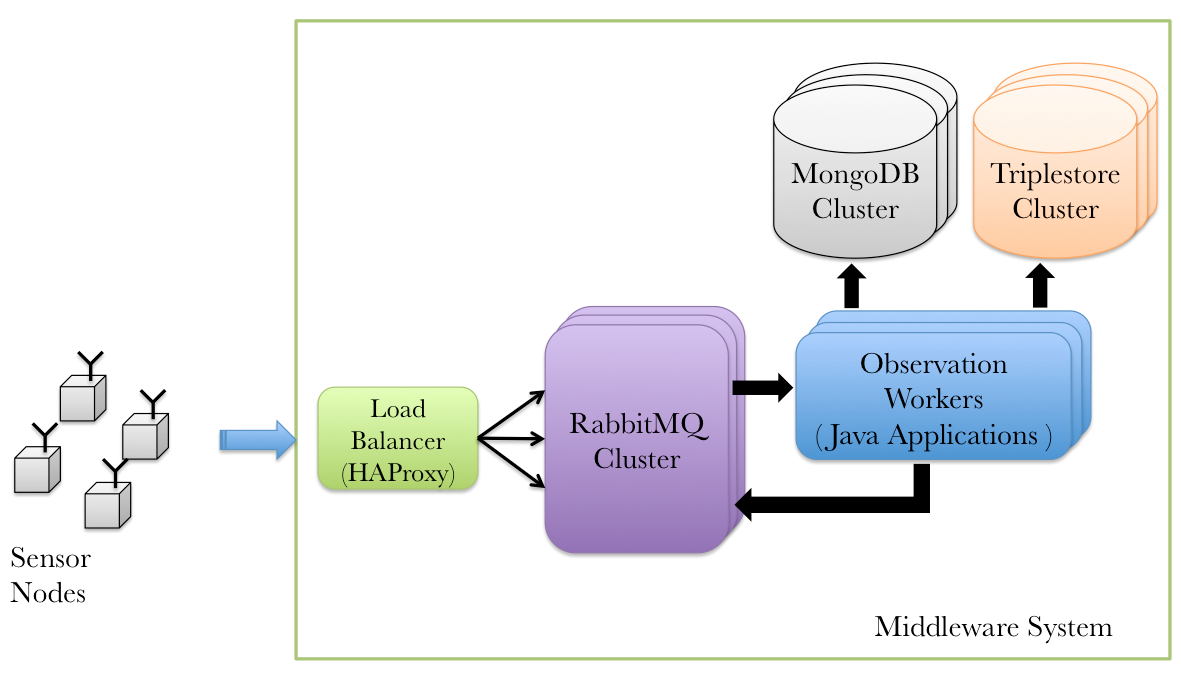
\includegraphics[width=130mm]{ir.png}
\caption{Simplified Architectural Model of Intelligent River\textsuperscript{\textregistered} Middleware }
\label{fig:ir}
\end{figure}

%Figure \ref{fig:ir} shows a simplified version of the architecture of Intelligent River\textsuperscript{\textregistered} Middleware system, where, sensor nodes are custom designed hardware devices that gather data from commodity sensor probes and transmit their observations to the load balancer, HAProxy \cite{haproxy} through wireless networks. The load balancer relays the observations to one of the nodes in a cluster of RabbitMQ \cite{rabbitmq} servers.

Figure \ref{fig:ir} shows a simplified version of the architecture of Intelligent River\textsuperscript{\textregistered} Middleware system, where, sensor nodes are custom designed hardware devices known as Motestacks \cite{motestack}, Load balancer is a physical server running HAProxy \cite{haproxy}, RabbitMQ cluster is a set of physical servers each running RabbitMQ \cite{rabbitmq}, Observation workers are a set of physical servers each running the custom developed Java applications, MongoDB cluster is a set of physical servers configured to run MongoDB in a sharded configuration \cite{mongosharding}, Triplestore cluster is a set of physical servers each running Apache Jena TDB \cite{tdb}.




Sensor nodes are custom designed hardware devices that gather data from commodity sensor probes. The sensor nodes transmit collected observations to the load balancer through wireless networks. The load balancer then relays the observations to any of the servers in the RabbitMQ cluster, which queues the observations to be fetched by the Observation worker applications. Observation worker applications are custom developed Java applications that fetch observations from the message queues in RabbitMQ, and performs (i) semantic analysis on the observations, (ii) persist both processed and unprocessed  observations onto MongoDB, (iii) persist the processed observations onto Triplestore, and (iv) publish the processed observation back to RabbitMQ for further analysis and visualizations.
















%Load balancer is a system running HAProxy \cite{haproxy}. 




 %custom designed sensor nodes transmit their observations to the load balancer in the middleware system through wireless networks. 
